\chapter{Erosion}
\label{chap:erosion}

\section{Introduction}
\label{sec:intro}
Solid-body erosion can be seen in everyday life in various physical processes.
It is commonly seen in areas where solid particles are carried in a pipe and
body part erosion of an aircraft due to the high-speed impact of particles. Due
to the continuous erosion, the conveying systems can result in total damage and
failure of the manufacturing system. Similarly, the aerodynamic performance of
the wings and other parts of an aircraft may reduce. An accurate study of solid
particle erosion can help improve the life and efficiency of such systems and
reduce maintenance costs. The experimental investigation is complex. In
addition, it may not provide detailed insight into the erosion process.

In the current chapter, we develop a numerical implementation to study the solid
particle erosion of a ductile target. We follow the numerical model proposed in
\citep{takaffoli2009finite,dong2016smoothed}. We utilize the numerical
techniques developed in the previous chapter to model solid-particle erosion. We
use the formulation proposed in \cref{chap:ctvf,chap:csph,chap:ctvf} to handle
the collision between the rigid bodies, elastic bodies and to model the dynamics
of the elastic structure of the target. We extend the developed numerical method
to simulate elastic-plastic behavior. A contact force model is used to handle
the collision between the impactor and the target. The complete work is made
open source and made available at
\url{https://github.com/dineshadepu/open_source_erosion}.

\begin{figure}[!htpb]
  \centering
  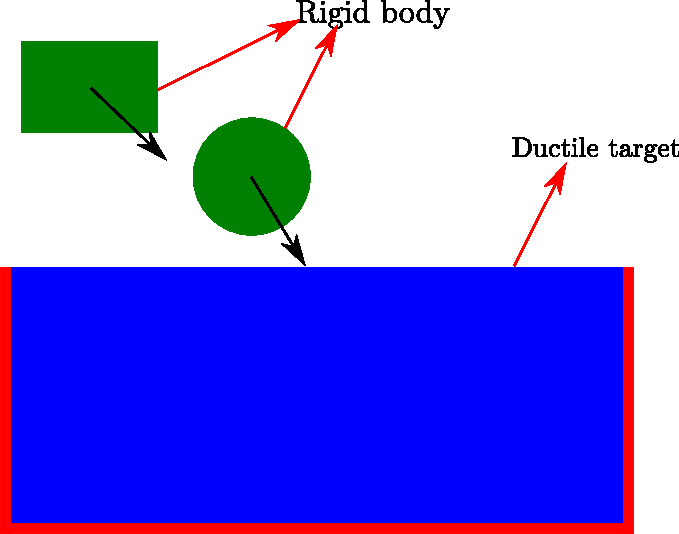
\includegraphics[width=0.5\textwidth]{images/erosion/images/intro/intro_description}
  \caption{A ductile target being impacted upon by two arbitrarily shaped rigid bodies.}
\label{fig:spe-intro}
\end{figure}
The primary targets of the current chapter are to develop an open-source framework
to handle solid-particle erosion in two and three dimensions. The developed
solver should be able to apply to problems involving multiple impacting
particles. The impacting particles could be interacting among themselves or not.
We study erosion of AL6061 due to a rotating solid particle impact at different
impacting velocities. An erosion of a ductile solid due to multiple square
particle impacts and erosion of a ductile solid due to multiple square
particle impacts where the square particles are allowed to collide among
themselves is studied. A representative example of multiple particles impacting
a ductile solid is shown in \cref{fig:spe-intro}.


\FloatBarrier%
\section{Numerical method}
\label{sec:erosion-numerical-method}
In the current section, equations governing the elastic-plastic behavior of the
ductile target are demonstrated. We utilize the scheme developed in
\cref{chap:ctvf} to model the elastic-plastic behavior of the solid. To model
the dynamics of the projectile, we employ the rigid body equations described in
\cref{chap:rfc}. The interaction between the projectiles and the target is
modeled using a contact force formulation described in
\cref{sec:contact-algorithm}. The contact force formulation is adapted to handle
the contact between the rigid and the elastic-plastic body.
\subsection{Discrete governing equations of the ductile target}
\label{chap-erosion:sec:discrete-governing-equations}
In addition to the equations of conservation of mass and momentum,
% of an elastic solid in \cref{sec:ctvf-sph-equations}, i.e., continuity and momentum,
we consider the energy equation to incorporate the plastic behavior of the
solid. The momentum equation is further modified to consider the contact due to
the external impact. The new modified equations are given as
\begin{multline}
\label{eqn:erosion-sph-momentum}
  \frac{\tilde{d}\ten{u}_{a}}{dt} = - \sum_{b \in A} m_b \left[
  \left(\frac{p_a}{\rho_a^2} + \frac{p_b}{\rho_b^2}\right) \ten{I} -
  \left(\frac{\teng{\sigma}^{'}_{a}}{\rho_a^2} +
  \frac{\teng{\sigma}^{'}_{b}}{\rho_b^2} + \Pi_{ab} \ten{I} \right) \right]  \cdot \nabla_{a} W_{ab} +
  \ten{g}_{a} + \frac{1}{m_a}\sum_{b \in B} \ten{F}^{\text{cont}}_{a \leftarrow b},
\end{multline}
\begin{equation}
\label{eqn:erosion-sph-energy}
  \frac{\tilde{d}{e}_{a}}{dt} = - \frac{1}{2} \sum_{b \in A} m_b
  \left(\frac{p_a}{\rho_a^2} + \frac{p_b}{\rho_b^2} + \Pi_{ab} \right)
  \left( \ten{v}_a - \ten{v}_b \right) \cdot \nabla_{a} W_{ab} +
  \frac{1}{\rho_a} \teng{\sigma}^{'}_{a} : \teng{\epsilon_a}.
\end{equation}
Here, $\ten{F}^{cont}_{a}$ is the force acting on particle $a$ due to contact
with the other rigid bodies as described in
\cref{sec:contact-algorithm}.

The plasticity behavior is incorporated based on the von Mises flow criterion.
According to the von Mises flow criterion, if the stress state exceeds the yield
surface, we bring back it the yield limit using the following equation,
\begin{equation}
  \sigma^{'}_{\alpha \beta} = \hat{f} \; \sigma^{'}^{*}_{\alpha \beta}.
\end{equation}
Here, $f_y = \min{(\sigma_y / \sigma^{'}^*, 1)}$, and
$\sigma^{'}^* = \sqrt{\frac{3}{2} \sigma^{'}^*_{\alpha \beta}
  \sigma^{'}^*_{\alpha \beta}}$. We use the Johnson-Cook constitutive
law \citep{johnson1983constitutive} to compute the yield
stress. Johnson-Cook model accounts for the effects of strain hardening, strain
rate hardening, and thermal softening. The flow stress is computed as
\begin{equation}
  \sigma_y = \bigg[A + B (\epsilon^{p}_{eff})^N \bigg]
  \bigg[1 + C \ln\bigg(\frac{\dot{\epsilon^{p}_{eff}}}{\dot{\epsilon_0}}\bigg) \bigg] \bigg[1 - (T^*)^M \bigg],
\end{equation}
where,
\begin{equation}
  \dot{\epsilon^{p}_{eff}} = \sqrt{\dot{\epsilon}_{\alpha \beta} \dot{\epsilon}_{\alpha \beta}},
\end{equation}
$A, B, N, \dot{\epsilon_{0}}, C, M$ are the Johnson-Cook parameters. $T^*$ is given as
\begin{equation}
  T^* = \frac{T - T_{ref}}{T_{melt} - T_{ref}},
\end{equation}
where $T_{ref}, T_{melt}, T$ are the room temperature, and melting point
temperature. $T$ is the temperature of the particle evolved using the energy
equation.

Finally, the new stress state is computed as
\begin{equation}
  \sigma_{\alpha \beta} = - P\delta_{\alpha \beta} + \sigma^{'}_{\alpha \beta}
\end{equation}
If a particle exceeds the yield limit, a plastic behaviour is identified and the
plastic strain increment is computed using
\begin{equation}
  \Delta \epsilon^{p}_{\alpha \beta} = (1 - \hat{f}) \sigma^{'}^{*}_{\alpha \beta} / 2 \mu,
\end{equation}
and the effective plastic strain increment is computed as,
\begin{equation}
  \Delta \epsilon^{p} = \frac{1}{3} \frac{1 - \hat{f}}{\mu}\sigma^{'}^{*}.
\end{equation}


The damage of the particle using the following equation.
\begin{equation}
  \epsilon_{\text{failure}} = [D_1 + D_2 \exp(D_3 \sigma^{*})]
  \bigg[ 1 + D_4 ln\big(\frac{\dot{\epsilon}_{eff}^p}{\dot{\epsilon}_{0}})\bigg]
  [1 + D_5 T^*]
\end{equation}
\begin{equation}
  D = \sum\frac{\Delta \epsilon_{eff}^p}{\epsilon_{\text{failure}}}
\end{equation}
If D exceeds $1$, then we make the particle's shear stress to $0$.



\subsection{Rigid body dynamics}
\label{chap-erosion:sec:rigid-body-dynamics}
From \cref{chap:rfc}, the governing equations of the rigid body are,
\begin{equation}
  \label{eq:balance_linear_mom}
  \frac{d \; (M \ten{v}_{cm})}{d t} = \sum_i \ten{F}_i,
\end{equation}
\begin{equation}
  \label{eq:balance_angular_mom}
  \frac{d \ten{L}}{d t} = \teng{\tau},
\end{equation}
where $\ten{F}_i = \ten{F}^{RB}_i + \ten{F}^{DS}_i$ are the forces acting on
particle $i$ due to the contact with the other rigid bodies ($\ten{F}^{RB}_a$)
and the ductile solid ($\ten{F}^{DS}_a$). Following
\cref{sec:contact-algorithm}, we compute the contact
forces on the ductile body and the rigid body. While computing the contact
force, we choose the ductile body as primary and the rigid projectile as
secondary body. This is because the boundary particles of the rigid body remain
constant throughtout the simulation, while the ductile target undergoes erosion and
the surface particles needs to be recomputed at every time instant if the target
erodes. The primary secondary differentiation is depicted in
\cref{fig:erosion-cnt-force-divide-bodies}.
\begin{figure}[!htpb]
  \centering
  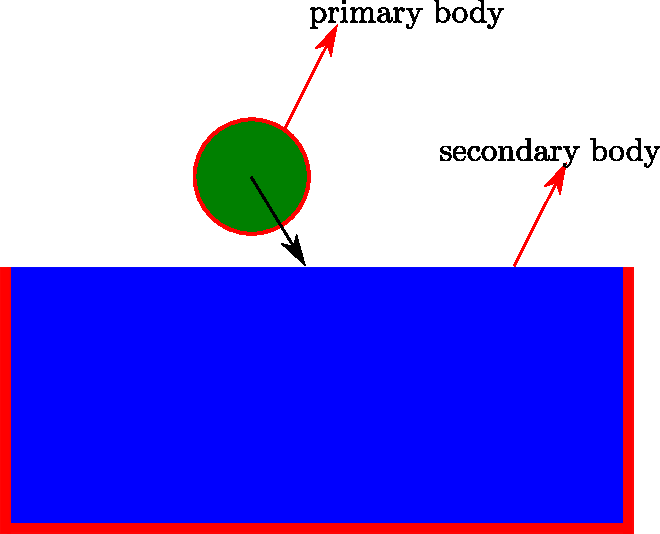
\includegraphics[width=0.5\textwidth]{images/erosion/images/contact_force/contact_force_divide}
  \caption{Bodies under collision divided into primary and secondary entities.}
\label{fig:erosion-cnt-force-divide-bodies}
\end{figure}


% ====================================================================================
% ====================================================================================
\FloatBarrier%
\section{Results}
\label{sec:erosion-results}
In the current section, the developed solver is applied to study the erosion of
a ductile solid under projectile impact. We considered erosion of AA6061
material due to the impact of a rotating spherical particle. Erosion of
AL6061-T6 material due to the impact of multiple square particles, where the
square particles are allowed to interact among themselves as one of the cases.


\FloatBarrier%
\subsection{A rigid sphere hitting a ductile specimen at different impact velocities}
\label{sec:erosion-vyas}
\begin{figure}[!htpb]
  \centering
  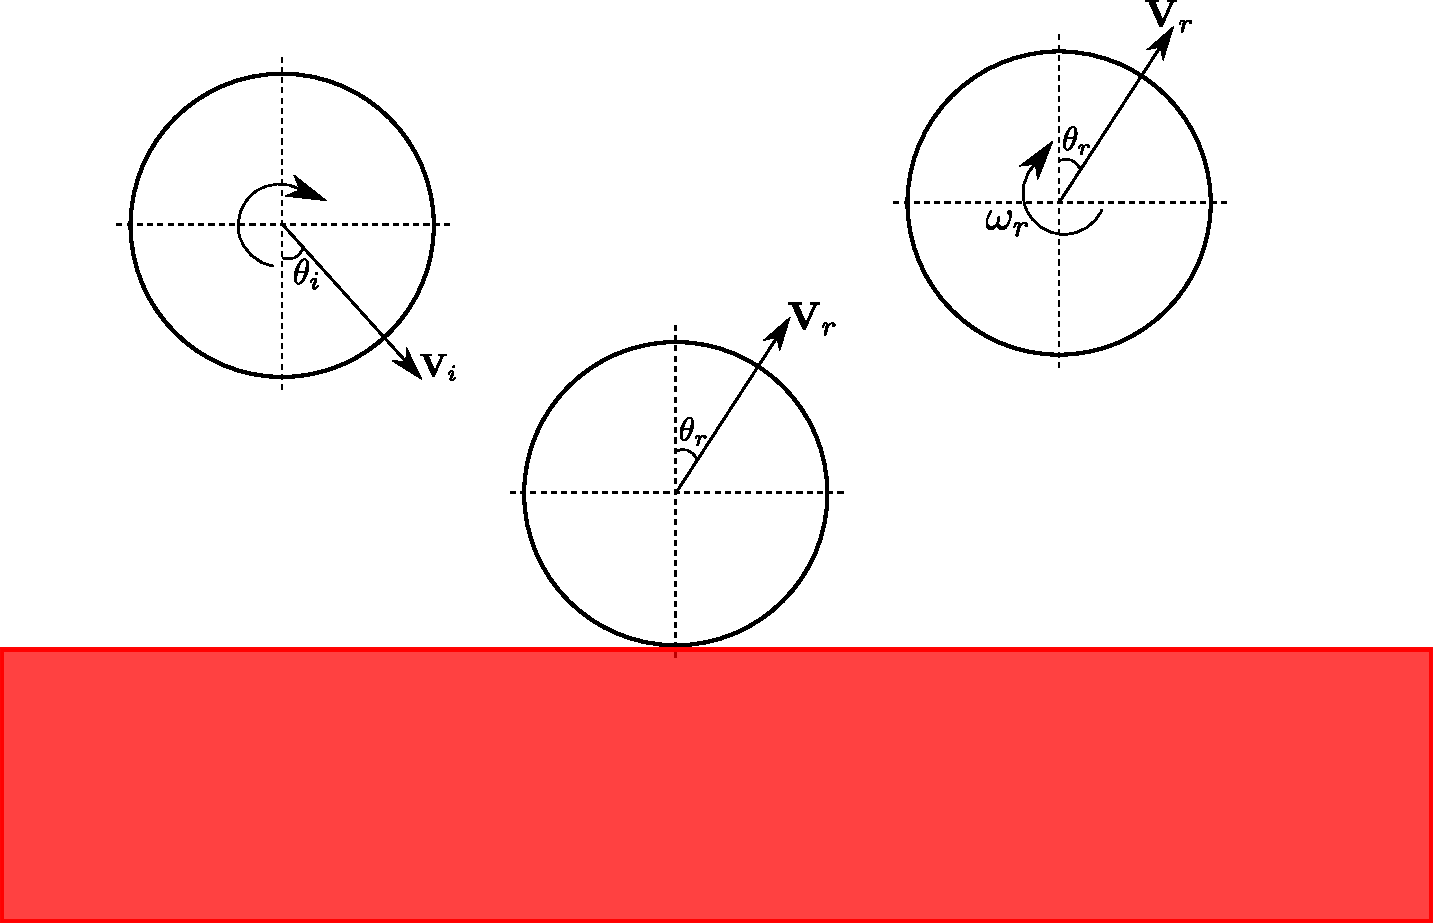
\includegraphics[width=0.6\textwidth]{images/erosion/images/vyas_2021_rebound_kinematics_3d/cao_drawing}
  \caption{A spherical particle impacting a ductile target at an impact angle
    with a velocity $\ten{V}_i$.}
\label{fig:results-cao-3d-erosion-schematic}
\end{figure}
In this test case, we study the erosion of AA6061 material due to the impact of
a rotating spherical particle. The model description is shown in
\cref{fig:results-cao-3d-erosion-schematic}. The sphere is assumed to be rigid
and the material properties as well as the numerical parameters used are
displayed in \cref{tab:sphere-target-impact,tab:sphere-target-impact-Johnson}.
The penetration depth of the ductile solid against the varying impact velocity
($\ten{V}_i$) with constant impact angle ($45$ degrees) is considered to
validate the developed solver. While in all the cases, the particle rotates with
a constant velocity of magnitude $1280$ radians per second. Further, this test is used to
demonstrate the capabilities of the developed solver to 3D solid-particle
erosion models. The experimental evaluation is carried out by
\cite{zang2022investigation}.
\begin{table}[!ht]
  \centering
  \caption{Numerical parameters and material properties for sphere impacting a target.}%
  \label{tab:sphere-target-impact}
  \begin{tabular}[!ht]{ll}
    \toprule
    Quantity & Values\\
    \midrule
    $E$, Young's modulus & $70$ GPa \\
    $\nu$, Poisson's ratio & $0.33$ \\
    $\rho$, density & $2700$ kg\,m\textsuperscript{-3} \\
    $\mu$, friction coefficient & $0.1$ \\
    Time of simulation & $0.25$ ms \\
    Resolution, $\delta x$ & $0.00153$ m\\
    Smoothing length factor, $h/\Delta x$ & 1.0\\
    gravity $[g_x, g_y, g_z]$ & $[0.0, -9.81, 0.0]$\\
    $k_r$, Normal stiffness coefficient & $10^{7}$ \\
    $k_f$, Tangential stiffness coefficient & $10^{5}$ \\
    $\text{Radius}$, Sphere radius & 5 $\times$ $10^{-3}$ m\\
    \bottomrule
  \end{tabular}
\end{table}
\begin{table}[!ht]
  \centering
  \begin{tabular}[!ht]{ll}
    \toprule
    Quantity & Values\\
    \midrule
    $A$ & $335$ MPa \\
    $B$ & $85$ MPa \\
    $C$ & $0.012$ \\
    $m$ & $1$ \\
    $n$ & $0.11$ \\
    $T_{ref}$ & $292$K \\
    $T_{melt}$ & $925$K \\
    \bottomrule
  \end{tabular}
  \caption{Johnson-Cook constitutive model parameters for the target.}%
  \label{tab:sphere-target-impact-Johnson}
\end{table}

\begin{figure}[!htpb]
  \centering
  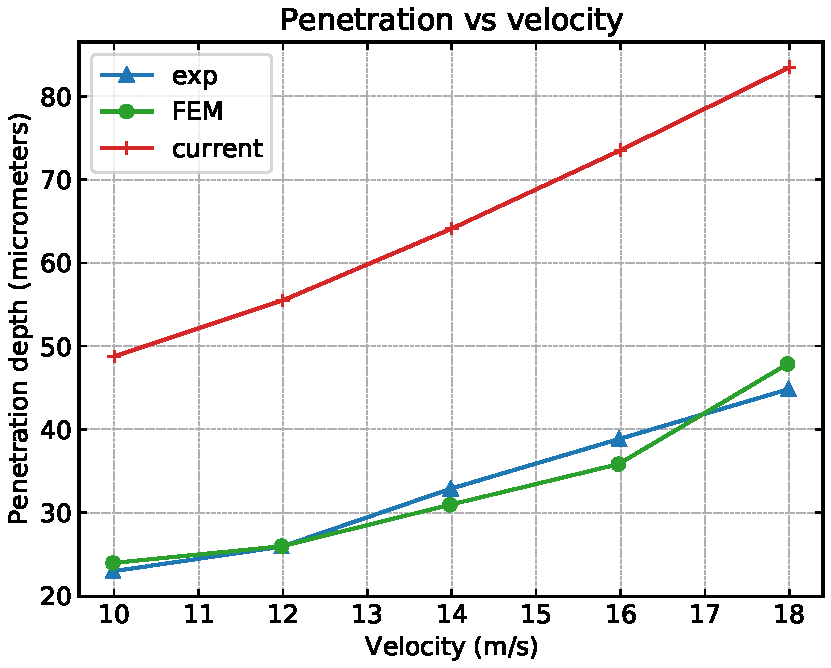
\includegraphics[width=0.6\textwidth]{figures/erosion/figures/cao_xuerui_2022_spherical_particle_impact_3d/penetration_vs_velocity}
  \caption{Variation of the penetration depth with the varying incident velocity
    magnitude compared against the experimental and numerical study with the
    current solve.}
  \label{fig:results-sphere-target-impact-vel-vs-depth}
\end{figure}
\Cref{fig:results-sphere-target-impact-vel-vs-depth} depicts the variation of
the depth against the incident velocity $\ten{V}_i$ of the current solver,
experimental and FEM result executed by \cite{zang2022investigation}. From
\Cref{fig:results-sphere-target-impact-vel-vs-depth}, we can see that the
current solver penetration depth increases as the velocity is increasing. A
similar trend is found with the experimental result as well. However, the
current solver is producing a higher penetration depth compared to the
experimental result.

\subsection{Solid-particle erosion due to multiple square particles: with no self
  interaction}
\label{sec:res:mpe-2}
In this test case, we study the erosion of AL6061-T6 material due to the
impact of multiple square particles. We assume the square particles do not
interact among themselves. The schematic of the test case is shown in
\cref{fig:mpe-2-pm}. This test is used to demonstrate the capabilities of the
developed an open-source solver for handling the erosion of a target due to multiple
non-interacting particles. The length of the square
\begin{figure}[!htpb]
  \centering
  \includegraphics[width=0.6\textwidth]{images/erosion/images/multi_body_erosion_example_2/physical_model.pdf}
  \caption{Schematic of ductile body being impacted by two non-interacting
    square particles.}
\label{fig:mpe-2-pm}
\end{figure}
particle is $4.780 \times 10^{-3}$ m and the target length and height are as
$4.780 \times 10^{-3}$ m and $14.340 \times 10^{-3}$ m respectively. At time
$t=0$ seconds, both the bodies are initialized with a velocity with the magnitude of
$255$ m\,s\textsuperscript{-1} and making an angle of $-60$ degrees with x-axis.
The square particle is oriented such that the hypotenuse makes an angle of $40$
degrees with the vertical line. The simulation is run for a total time of $40$
microseconds. We use two computational models to study the multi-particle
erosion problem. One where the rigid body is represented using the boundary
particles, and in another case, the complete democratization of the rigid body
is utilized. These computational models are shown in
\cref{fig:mpe-2-cm}.
\begin{figure}[!htpb]
  \centering
  \begin{subfigure}{0.48\textwidth}
    \centering
    \includegraphics[width=\textwidth]{images/erosion/images/multi_body_erosion_example_2/computational_model_1.pdf}
    \subcaption{}
  \end{subfigure}
  \begin{subfigure}{0.48\textwidth}
    \centering
    \includegraphics[width=\textwidth]{images/erosion/images/multi_body_erosion_example_2/computational_model_2.pdf}
    \subcaption{}
  \end{subfigure}
  \caption{Computational models considered in the current work to simulate the
    erosion of ductile solid due to multiple non-interacting square particles:
    (a) computational model 1: Square particle represented using boundary particles alone,
    (b) computational model 2: Square particle represented with full particles.}
\label{fig:mpe-2-cm}
\end{figure}
The material properties and the numerical parameters are listed in
\cref{tab:sphere-target-impact,tab:sphere-target-impact-Johnson}.
\begin{table}[!ht]
  \caption{Numerical parameters and material properties for sphere impacting a target.}%
  \label{tab:mpe-2-mat-prop}
  \centering
  \begin{tabular}[!ht]{ll}
    \toprule
    Quantity & Values\\
    \midrule
    $E$, Young's modulus & $70$ GPa \\
    $\nu$, Poisson's ratio & $0.33$ \\
    $\rho$, density & $2700$ kg\,m\textsuperscript{-3} \\
    $\mu$, friction coefficient & $0.1$ \\
    Time of simulation & $0.25$ ms \\
    Resolution, $\delta x$ & $0.00153$ m\\
    Smoothing length factor, $h/\Delta x$ & 1.0\\
    gravity $[g_x, g_y, g_z]$ & $[0.0, -9.81, 0.0]$\\
    $k_r$, Normal stiffness coefficient & $10^{7}$ \\
    $k_f$, Tangential stiffness coefficient & $10^{5}$ \\
    $\text{Radius}$, Sphere radius & 5 $\times$ $10^{-3}$ m\\
    \bottomrule
  \end{tabular}
\end{table}
\begin{table}[!ht]
  \caption{Johnson-Cook constitutive model parameters for the target.}%
  \label{tab:mpe-2-john-prop}
  \centering
  \begin{tabular}[!ht]{ll}
    \toprule
    Quantity & Values\\
    \midrule
    $A$ & $335$ MPa \\
    $B$ & $85$ MPa \\
    $C$ & $0.012$ \\
    $m$ & $1$ \\
    $n$ & $0.11$ \\
    $T_{ref}$ & $292$K \\
    $T_{melt}$ & $925$K \\
    \bottomrule
  \end{tabular}
\end{table}



\begin{figure}[!htpb]
  \centering
  \begin{subfigure}{0.48\textwidth}
    \centering
    \includegraphics[width=\textwidth]{figures/erosion/figures/multi_body_erosion_example_2/border_particles_no_self_intersection/all_bodies_time0.pdf}
    \subcaption{}
    \label{fig:mpe-2-border-a}
  \end{subfigure}
  \begin{subfigure}{0.48\textwidth}
    \centering
    \includegraphics[width=\textwidth]{figures/erosion/figures/multi_body_erosion_example_2/border_particles_no_self_intersection/all_bodies_time1.pdf}
    \subcaption{}
    \label{fig:mpe-2-border-b}
  \end{subfigure}
  \caption{Erosion of a ductile target due to the impact of two non-interacting
    square particles with computational model 1.}
\label{fig:mpe-2-border}
\end{figure}
\Cref{fig:mpe-2-border} shows the snapshots of the square particles, including
the target for the non-interacting square particles case. Here, the simulation is
carried out using computational model 1, where the target and the body are
discretized into $8476$ particles. \Cref{fig:mpe-2-border-a} shows the square
particle and the target during the first impact. \Cref{fig:mpe-2-border-b} shows
the second particle impacting the target, and from the figure, we can see the
chip separation. From \cref{fig:mpe-2-border-b} we can also see the material
eroded due to the first particle impact flying away. Since, in the current case,
we do not consider the mutual interaction of the impacting bodies, in
\cref{fig:mpe-2-border-b}, we see the impacting square particles overlapping.


\Cref{fig:mpe-2-full} shows the snapshots for computational model 2. The target
and the body are discretized into $12708$ particles in the current case. From
\cref{fig:mpe-2-full,fig:mpe-2-border}, we can see that the both computational
models result in same erosion of the target, which is verified qualitatively by
comparing the eroded regions of of the target. For a quantitative validation, we
compare the y component of the center of mass of the bottom square particle with
time, when simulated using both the models in \cref{fig:mpe-2-ycom-vs-t}. From
\cref{fig:mpe-2-ycom-vs-t}, we can see that both the computational models give
the same result. Though both the models result in same erosion of the target,
however, computational model 1 is $2.3$ times faster than computational model 2.
This is due to boundary particle representation in the 1st model. A clearer
description is shown in \cref{table:mpe-2-time-comparison}.
\begin{figure}[!htpb]
  \centering
  \begin{subfigure}{0.48\textwidth}
    \centering
    \includegraphics[width=\textwidth]{figures/erosion/figures/multi_body_erosion_example_2/all_particles_no_self_intersection/all_bodies_time0.pdf}
    \subcaption{}
    \label{fig:mpe-2-full-a}
  \end{subfigure}
  \begin{subfigure}{0.48\textwidth}
    \centering
    \includegraphics[width=\textwidth]{figures/erosion/figures/multi_body_erosion_example_2/all_particles_no_self_intersection/all_bodies_time1.pdf}
    \subcaption{}
    \label{fig:mpe-2-full-b}
  \end{subfigure}
  \caption{Erosion of a ductile target due to the impact of two non-interacting
    square particles with computational model 2.}
\label{fig:mpe-2-full}
\end{figure}
\begin{figure}[!htpb]
  \centering
  \includegraphics[width=0.6\textwidth]{figures/erosion/figures/multi_body_erosion_example_2/no_self_intersection_y_com_vs_time.pdf}
  \caption{Variation of the y component of the center of mass of body 1 with
    time, for the solid particle erosion test case, with non-interacting particles.}
\label{fig:mpe-2-ycom-vs-t}
\end{figure}
\begin{table}[!htpb]
\centering
\begin{tabular}{c c c c c}
  \hline
  Model & No. particles & Time taken & Scale up  \\
  \hline
  Computational model 1 & $8476$ & $200.36$ sec & $2.3$ \\
  Computational model 2 & $12708$ & $460.21$ sec & 1 \\
\end{tabular}
\caption{CPU time comparison of computational model 1 and computational model 2
  for solid particle erosion for non-interacting particles.}
\label{table:mpe-2-time-comparison}
\end{table}

% ====================================================================================
% ====================================================================================
\FloatBarrier%
\subsection{Solid-particle erosion due to multiple square particles: with
  self interaction}
\label{sec:erosion-multiple-impact-self-interact}
In this test case, we study the erosion of AL6061-T6 material due to multiple
square particle impacts. In contrast to the previous section, we allow square
particles to interact among themselves. The schematic of the colliding particles
and the target is shown in \cref{fig:mpe-1-pm}. The length of the square
\begin{figure}[!htpb]
  \centering
  \includegraphics[width=0.6\textwidth]{images/erosion/images/multi_body_erosion_example_1/physical_model.pdf}
  \caption{Schematic of ductile body being impacted by two interacting square
    particles.}
\label{fig:mpe-1-pm}
\end{figure}
particle, the target length, and the height are as same as in the previous test
case. At time $t=0$ seconds, body $2$ is initialized with a velocity with the
magnitude of $255$ m\,s\textsuperscript{-1} and making an angle of $-45$ degrees
with x-axis and body 1 with same velocity magnitude, making an angle of $-90$
with the x-axis. Both the square particles are oriented such that the hypotenuse
makes an angle of $90$ degrees with the vertical line as shown in
\cref{fig:mpe-1-pm}. The simulation is run for a total time of $40$
microseconds. We use two computational models to study the problem similar to
the previous test case. These computational models are shown in
\cref{fig:mpe-1-cm}.
\begin{figure}[!htpb]
  \centering
  \begin{subfigure}{0.48\textwidth}
    \centering
    \includegraphics[width=\textwidth]{images/erosion/images/multi_body_erosion_example_1/computational_model_1.pdf}
    \subcaption{}
  \end{subfigure}
  \begin{subfigure}{0.48\textwidth}
    \centering
    \includegraphics[width=\textwidth]{images/erosion/images/multi_body_erosion_example_1/computational_model_2.pdf}
    \subcaption{}
  \end{subfigure}
  \caption{Computational models considered to simulate the erosion of ductile
    solid due to multiple interacting square particles: (a) computational model
    1: Square particle represented using boundary particles alone, (b)
    computational model 2: Square particle represented with full particles.}
\label{fig:mpe-1-cm}
\end{figure}
The material properties and the numerical parameters are listed in
\cref{tab:sphere-target-impact,tab:sphere-target-impact-Johnson}.


\begin{figure}[!htpb]
  \centering
  \begin{subfigure}{0.48\textwidth}
    \centering
    \includegraphics[width=\textwidth]{figures/erosion/figures/multi_body_erosion_example_1/border_particles_self_intersection/all_bodies_time0.pdf}
    \subcaption{}
    \label{fig:mpe-1-border-a}
  \end{subfigure}
  \begin{subfigure}{0.48\textwidth}
    \centering
    \includegraphics[width=\textwidth]{figures/erosion/figures/multi_body_erosion_example_1/border_particles_self_intersection/all_bodies_time1.pdf}
    \subcaption{}
    \label{fig:mpe-1-border-b}
  \end{subfigure}
  \caption{Erosion of a ductile target due to the impact of two interacting
    square particles with computational model 1.}
\label{fig:mpe-1-border}
\end{figure}
\begin{figure}[!htpb]
  \centering
  \begin{subfigure}{0.48\textwidth}
    \centering
    \includegraphics[width=\textwidth]{figures/erosion/figures/multi_body_erosion_example_4/hollow_body/all_bodies_time0.pdf}
    \subcaption{}
    \label{fig:mpe-4-border-a}
  \end{subfigure}
  \begin{subfigure}{0.48\textwidth}
    \centering
    \includegraphics[width=\textwidth]{figures/erosion/figures/multi_body_erosion_example_4/hollow_body/all_bodies_time1.pdf}
    \subcaption{}
    \label{fig:mpe-4-border-b}
  \end{subfigure}
  \caption{Erosion of a ductile target due to the normal impact of a
    square particle.}
  \label{fig:mpe-4-border}
\end{figure}
\Cref{fig:mpe-1-border} shows the snapshot of the target during the impact for
the computational model 1. \Cref{fig:mpe-1-border-a} shows the penetration of
body $1$ into the ductile target, and initial impact of the body $2$ with body
$1$. \Cref{fig:mpe-1-border-b} shows the snapshot after body $1$ loses the
contact with the target. \Cref{fig:mpe-4-border} shows the snapshot of the
target during the impact for the computational model 1 with a single square
particle. From \cref{fig:mpe-4-border}, we can see that the impacting body
erodes the target symmetrically and after losing contact it moves away from the
away without acquiring a rotation. However, for the two square particle impact
case, the material is eroded more from the right side, this is due to the second
square particle impact, this can be seen in \cref{fig:mpe-1-border}.

We repeat the same experiment with computational model 2. The erosion of the
ductile solid with computational model 2 is shown in \cref{fig:mpe-1-full}. From
\cref{fig:mpe-1-full,fig:mpe-1-border}, we can see that both the computational
models results in same erosion pattern. For quantitatively validation for the
similarity, we plot center of mass of the 1st body with time in
\cref{fig:mpe-1-ycom-vs-t}. From \cref{fig:mpe-1-ycom-vs-t}, we can see that
both 1 behaves same in both the computational models. The performance comparison
of the proposed computational models are shown in
\cref{table:mpe-1-time-comparison}.
\begin{figure}[!htpb]
  \centering
  \begin{subfigure}{0.48\textwidth}
    \centering
    \includegraphics[width=\textwidth]{figures/erosion/figures/multi_body_erosion_example_1/all_particles_self_intersection/all_bodies_time0.pdf}
    \subcaption{}
    \label{fig:mpe-1-full-a}
  \end{subfigure}
  \begin{subfigure}{0.48\textwidth}
    \centering
    \includegraphics[width=\textwidth]{figures/erosion/figures/multi_body_erosion_example_1/all_particles_self_intersection/all_bodies_time1.pdf}
    \subcaption{}
    \label{fig:mpe-1-full-b}
  \end{subfigure}
  \caption{Erosion of a ductile target due to the impact of two interacting
    square particles with computational model 2.}
\label{fig:mpe-1-full}
\end{figure}
\begin{figure}[!htpb]
  \centering
  \includegraphics[width=0.6\textwidth]{figures/erosion/figures/multi_body_erosion_example_1/self_intersection_y_com_vs_time.pdf}
  \caption{Variation of the y component of the center of mass of body 1 with
    time, for the solid particle erosion test case, with interacting particles.}
\label{fig:mpe-1-ycom-vs-t}
\end{figure}


\begin{table}[!htpb]
\centering
\begin{tabular}{c c c c c}
  \hline
  Model & No. particles & Time taken & Scale up  \\
  \hline
  Computational model 1 & $8476$ & $239.36$ sec & $1.956$ \\
  Computational model 2 & $12708$ & $468.21$ sec & 1 \\
\end{tabular}
\caption{CPU time comparison of computational model 1 and computational model 2
  for solid particle erosion for interacting particles.}
\label{table:mpe-1-time-comparison}
\end{table}
The demonstrated test cases show that the developed software can handle the
modeling erosion of a body in 2 and 3 dimensions. Further, we verified that the
representation of projectiles with border particles reduces the time of
computation. We established the current framework for handling erosion due to
multiple particle impacts.



\FloatBarrier%
\section{Summary}
In this chapter we studied erosion of a ductile target due to a solid particle
impact. The solver developed in \cref{chap:ctvf} is further extended to handle
plastic behaviour. A von Mises criterion is followed to model the plasticity. A
Johnson-Cook constitutive model is employed to compute the yield stress of the
solid. The dynamics of projectile is modeled following the rigid body dynamics
formulation proposed in \cref{chap:rfc}. The interaction between the target and
the projectile is modeled using the contact force formulation described in
\cref{sec:contact-algorithm}. A 3D case where erosion of the target due to a
rotating spherical particles, erosion of a target due to multiple impact of
square particles, where the impacting particles are allowed to self interact is
considered to demonstrate the suite of problems the developed framework can handle.

The deformation of AA6061 target due to a spherical impact is studied with different
impacting particle velocities. We are able to capture the trend of the
deformation of the target as the variation of the projectile velocity, where we
see an increased penetration depth with an increase in velocity. We have
compared the current penetration against the impact velocity with the
finite element method results and the experimental one. We were able to get the
variation of the penetration with a velocity similar to the experimental and the
FEM simulation model. A two-dimensional study is carried out on the erosion of
targets due to the impact of multiple square particles. Erosion of AL6061-T6 due
to multiple impacts of a square particle is studied. Here, we were able to see
the gouging, chip separation, and lip formation due to the particle impact. Two
computational models are considered, where we have represented the rigid body
using the boundary particles alone, and in another case, full discretization of
the rigid body is used. The current implementation of rigid body dynamics allows
us to model the rigid body using just boundary particles by using body and
global frame axis representation. We compared the performance of both the
formulation in multiple square particle collision cases. We have seen upto twofold
performance improvement using boundary representation than full discretization.
We have made the current implementation open-source, and all the study cases fully
reproducible.
